%!TEX root = ./proposta3.tex

Para explorar e validar a proposta deste trabalho, foram realizados experimentos de acordo com as métricas especificadas por \cite{4600003}, primeiramente, foi avaliado o impacto da mitigação de DDoS em tempo de resposta e, em seguida, em relação à taxa de resposta e \emph{overhead}. 
%
%
Como pode ser observado na Figura \ref{fig:blacklistSecs}, o uso da arquitetura proposta reduziu o tempo de resposta às requisições legítimas em comparação ao gráfico à direita, que mostra o tempo gasto para atender o mesmo número de requisições originadas sem o nosso mecanismo. Tal comportamento se deve ao fato de que com o uso da solução, uma \emph{blacklist} impedirá a aplicação de responder o mesmo cliente múltiplas vezes, ainda assim garantindo que o cliente legítimo seja capaz de atingir a nova instância.

\begin{figure}[h!]
\centering
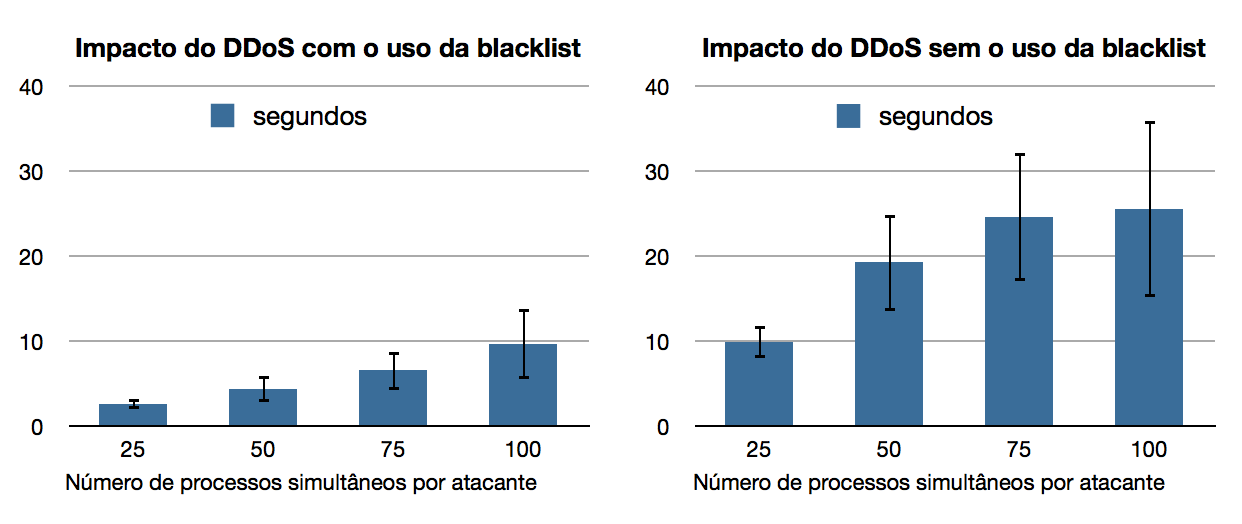
\includegraphics[width=0.76\textwidth]{images/blacklistSecs.png}
\caption{Tempo de resposta para clientes legítimos}
\label{fig:blacklistSecs}
\end{figure}




Outra métrica avaliada é a taxa de páginas solicitadas recebidas com sucesso (Figura~\ref{fig:blacklistTxResp}). Observaram-se  perdas apenas quando não foram utilizadas a filtragem pela \emph{blacklist} e conseqüente redirecionamento. Nestes casos, a aplicação envia uma resposta ao atacante, que descarta esta resposta de imediato, dando continuidade ao ataque. Nota-se que a taxa de entrega sem o uso da \emph{blacklist} é afetada pela ocorrência de \emph{timeouts}.


\begin{figure}[h!]
\centering
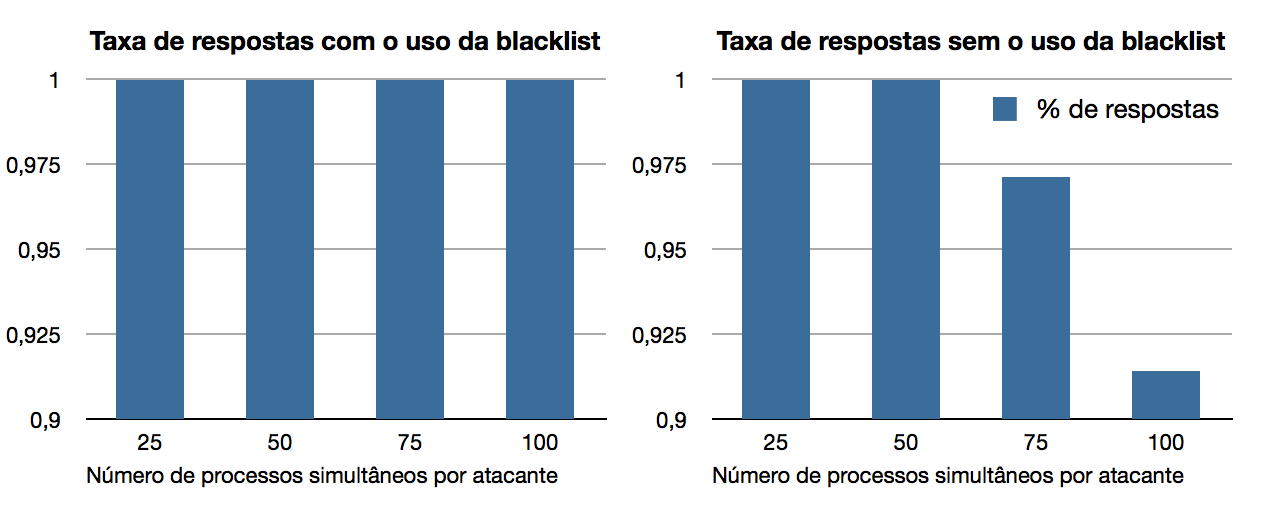
\includegraphics[width=0.76\textwidth]{images/blacklistTxResp.png}
\caption{Tempo de resposta para clientes legítimos}
\label{fig:blacklistTxResp}
\end{figure}
% 
% Por fim, foi analisado o \emph{overhead} causado pela arquitetura proposta em relação a execução normal da aplicação. O gráfico %\ref{fig:overhead}
% demonstra que a solução causa um impacto insignificante na execução. A parte verde do gráfico denota o tempo gasto em $ms$ pelo enfileiramento das requisições dos atacantes. O \emph{overhead} causado pelo mecanismo proposto é observado na linha preta, acima da superfície verde. Neste gráfico, pode-se notar 4 patamares diferentes no tempo gasto para o enfileiramento das requisições. Durante o tempo entre 11:10 e 11:17, os nós atacantes estavam executando 100 instâncias do \emph{script de ataque.} No instante entre 11:17 e 11:30, 75 instâncias, entre 11:30 e 11:40, 50 instâncias e, por fim, entre 11:40 e 11:45, 25 instâncias.

%\begin{figure}[h!]
%  \centering
%  \includegraphics[height=8cm]{images/overhead-p1.pdf}
%  \includegraphics[height=8cm]{images/overhead-p2.pdf}
%  \caption{Overhead em $ms$ causado pela solução}
%	\label{fig:overhead}
%\end{figure}


